\begin{tikzpicture}
  \begin{scope}[yshift=0cm]
    \tikzstyle{graph_node}=[circle,minimum size=0.014\textwidth,inner sep=0pt, fill=camlightblue]
    \def \radius {0.045\textwidth}
    \begin{scope}[xshift=0cm]
      \foreach \s in {1,...,10}
      {
        \node[draw, graph_node] (N\s) at ({360/10 * (\s - 1) + 90}:\radius) {\s};
      }   
      \path (N2) edge (N6);
      \path (N4) edge (N9);
      \path (N5) edge (N6);
      \path (N5) edge (N8);
      \path (N7) edge (N8);
      \path (N8) edge (N9);
      \path (N8) edge (N10);
      \path (N9) edge (N10);
    \end{scope}
    \begin{scope}[xshift=0.14\textwidth]
      \def \s {1}
      \node[draw, graph_node] (N\s) at ({360/10 * (\s - 1) + 90}:\radius) {2};
      \def \s {2}
      \node[draw, graph_node] (N\s) at ({360/10 * (\s - 1) + 90}:\radius) {7};
      \def \s {3}
      \node[draw, graph_node] (N\s) at ({360/10 * (\s - 1) + 90}:\radius) {6};
      \def \s {4}
      \node[draw, graph_node] (N\s) at ({360/10 * (\s - 1) + 90}:\radius) {5};
      \def \s {5}
      \node[draw, graph_node] (N\s) at ({360/10 * (\s - 1) + 90}:\radius) {3};
      \def \s {6}
      \node[draw, graph_node] (N\s) at ({360/10 * (\s - 1) + 90}:\radius) {1};
      \def \s {7}
      \node[draw, graph_node] (N\s) at ({360/10 * (\s - 1) + 90}:\radius) {10};
      \def \s {8}
      \node[draw, graph_node] (N\s) at ({360/10 * (\s - 1) + 90}:\radius) {8};
      \def \s {9}
      \node[draw, graph_node] (N\s) at ({360/10 * (\s - 1) + 90}:\radius) {4};
      \def \s {10}
      \node[draw, graph_node] (N\s) at ({360/10 * (\s - 1) + 90}:\radius) {9};
      \path (N2) edge (N6);
      \path (N4) edge (N9);
      \path (N5) edge (N6);
      \path (N5) edge (N8);
      \path (N7) edge (N8);
      \path (N8) edge (N9);
      \path (N8) edge (N10);
      \path (N9) edge (N10);
    \end{scope}
    \begin{scope}[xshift=0.07\textwidth]
      \node[inner sep=0,text width=0.13\textwidth, text centered,font=\Huge] (note1) at (0,0) {
         $\equiv$};
    \end{scope}
  \end{scope}
  \begin{scope}[yshift=-0.14\textwidth]
    \begin{scope}[xshift=0cm]
      \node [mybox] (box){
        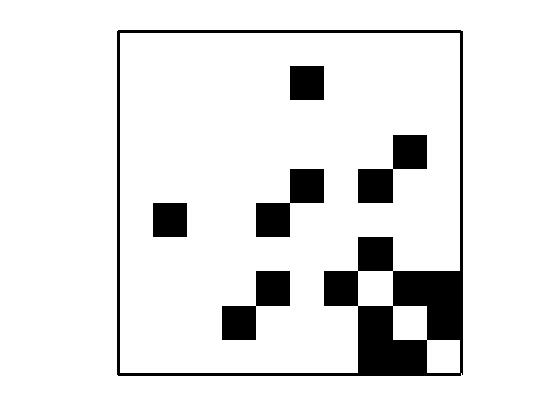
\includegraphics[width=0.15\textwidth]{../misc/adj.png}
      };
    \end{scope}
    \begin{scope}[xshift=0.14\textwidth]
      \node [mybox] (box){
        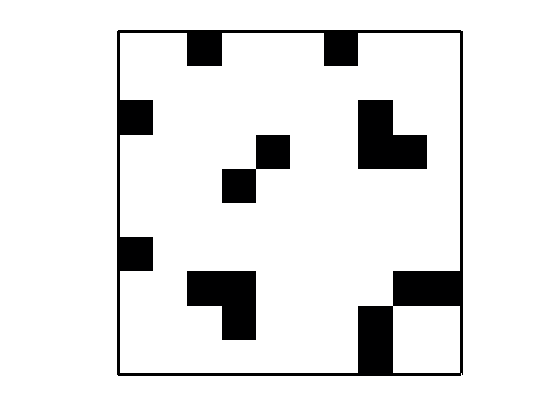
\includegraphics[width=0.15\textwidth]{../misc/adj_perm.png}
      };
    \end{scope}
    \begin{scope}[xshift=0.07\textwidth]
      \node[inner sep=0,text width=0.13\textwidth, text centered,font=\Huge] (note1) at (0,0) {
         $\equiv$};
    \end{scope}
  \end{scope}
\end{tikzpicture}
